\chapter{HUMAN S100A5 BINDS CA2+ AND CU2+ INDEPENDENTLY}

\section{Author Contributions}
Lucas Wheeler and Michael Harms conceived the study and designed the experiments. Lucas Wheeler performed all experiments and data analysis. Michael Harms secured funding for the work. Lucas Wheeler wrote the manuscript and generated the figures. Both authors have read and approved the manuscript. 

\section{Abstract}

S100A5 is a calcium binding protein found in a small subset of amniote
tissues. Little is known about the biological roles of S100A5, but
it may be involved in inflammation and olfactory signaling. Previous
work indicated that S100A5 displays antagonism between binding of
Ca\textsuperscript{2+} and Cu\textsuperscript{2+} ions---one of the
most commonly cited features of the protein. We set out to characterize
the interplay between Ca\textsuperscript{2+} and Cu\textsuperscript{2+} 
binding by S100A5 using isothermal titration calorimetry (ITC), circular
dichroism spectroscopy (CD), and analytical ultracentrifugation (AUC). 

We found that human S100A5 is capable of binding both Cu\textsuperscript{2+} 
and Ca\textsuperscript{2+} ions simultaneously. The wildtype protein
was extremely aggregation-prone in the presence of Cu\textsuperscript{2+} 
and Ca\textsuperscript{2+}. A Cys-free version of S100A5, however,
was not prone to precipitation or oligomerization. Mutation of the
cysteines does not disrupt the binding of either Ca\textsuperscript{2+} 
or Cu\textsuperscript{2+} to S100A5. In the Cys-free background,
we measured Ca\textsuperscript{2+} and Cu\textsuperscript{2+} binding
in the presence and absence of the other metal using ITC. Saturating
concentrations of Ca\textsuperscript{2+} or Cu\textsuperscript{2+} 
do not disrupt the binding of one another. Ca\textsuperscript{2+} 
and Cu\textsuperscript{2+} binding induce structural changes in S100A5,
which are measurable using CD spectroscopy. We show via sedimentation
velocity AUC that the wildtype protein is prone to the formation of
soluble oligomers, which are not present in Cys-free samples.

S100A5 can bind Ca\textsuperscript{2+} and Cu\textsuperscript{2+} 
ions simultaneously and independently. This observation is in direct
contrast to previously-reported antagonism between binding of Cu\textsuperscript{2+} 
and Ca\textsuperscript{2+} ions. The previous result is likely due
to metal-dependent aggregation. Little is known about the biology
of S100A5, so an accurate understanding of the biochemistry is necessary
to make informed biological hypotheses. Our observations suggest the
possibility of independent biological functions for Cu\textsuperscript{2+} 
and Ca\textsuperscript{2+} binding by S100A5.


\section{Background}
S100A5 is a member of the calcium-binding S100 protein family. The
protein is primarily homodimeric and is capable of binding one Ca\textsuperscript{2+} ion
each at it's EF-hand and pseudo-EF-hand sites \cite{bertini_solution_2009,kim_biophysical_2017}.
S100A5 undergoes a notable conformational change upon calcium-binding,
resulting in the rotation and extension of a helix \cite{bertini_solution_2009}.
This Ca\textsuperscript{2+}-driven exposure of a hydrophobic surface
is the primary mode of signal transduction in the S100 proteins \cite{santamaria-kisiel_calcium-dependent_2006}.
Through interactions with metals and protein targets, S100s play a
variety of biological roles including control of cell proliferation,
inflammatory signalling, and antimicrobial activity \cite{leclerc_binding_2009,heizmann_new_nodate,zhu_s100a16_2016,donato_functions_2013}. 

S100A5 is expressed primarily in the olfactory bulb and olfactory
sensory neurons (OSNs). Its expression is dramatically upregulated
by odor stimulation \cite{fischl_activity-dependent_2014,schafer_brain_2000,teratani_restricted_2002}.
It has been proposed that S100A5 is actively involved in olfactory
signalling due to its expression profile \cite{schafer_brain_2000}.
Expression of the protein has also been observed in a small number
of other tissues \cite{teratani_restricted_2002}. It is used as
a bio-marker for several types of brain cancers and inflammatory disorders
and appears to be involved in inflammation via activation of RAGE
\cite{cho_pentamidine_2016,kim_biophysical_2017,hancq_s100a5:_2004}.
Genetic work on S100A5 has been minimal, which has limited our understanding
of its biological roles.

The first biochemical study of human S100A5 identified it as a novel
Ca\textsuperscript{2+}, Cu\textsuperscript{2+}, and Zn\textsuperscript{2+} 
binding protein \cite{schafer_brain_2000}. The authors used flow-dialysis
to measure binding of the metal ions to the protein and concluded
that S100A5 is capable of binding four Ca\textsuperscript{2+} ions,
four Cu\textsuperscript{2+} ions, and two Zn\textsuperscript{2+} 
ions per homodimer. One of the most striking observations of that
study was the strong antagonism between the binding of Cu\textsuperscript{2+} 
and Ca\textsuperscript{2+} ions to the protein. This feature is one
of the most highly cited aspects of S100A5. Because little is known
about the protein, this fact is present in descriptions found across
databases such as Uniprot, NCBI, Wikigenes, and Genecards \cite{noauthor_wikigenes_nodate,noauthor_s100a5_nodate,noauthor_s100a5_nodate-1}.
While most S100s are capable of binding transition metal ions, antagonism
with binding of Ca\textsuperscript{2+} is not known outside the S100A5
lineage. Thus, this unique feature of S100A5 provoked speculation
about its possible biological implications \cite{schafer_brain_2000,moroz_role_2010}.
It was suggested that S100A5 might act as a Cu\textsuperscript{2+} 
and Ca\textsuperscript{2+} regulated signal during olfaction or as
a Cu\textsuperscript{2+} sink to accommodate high Cu\textsuperscript{2+} 
concentrations in the olfactory bulb \cite{schafer_brain_2000}. 

We sought to characterize this presumably important feature of S100A5
in more detail. Previously, we characterized the binding of Cu\textsuperscript{2+} 
and Zn\textsuperscript{2+} to a large number of S100 proteins including
S100A5 \cite{wheeler_multiple_2016}. Via ITC competition experiments,
we established that these two metals bind at different sites on the
protein and do not compete for binding \cite{wheeler_multiple_2016}.
We found that mutation of Cys43 and Cys79 lead to a loss of Zn\textsuperscript{2+} 
binding. In contrast neither of these residues was necessary for binding
of Cu\textsuperscript{2+}. Due to the original report of Ca\textsuperscript{2+} /Cu\textsuperscript{2+} 
antagonism we suspected that Ca\textsuperscript{2+} and Cu\textsuperscript{2+} 
may compete for the same sites on S100A5. 

Here we report our study of the interplay between Ca\textsuperscript{2+} 
and Cu\textsuperscript{2+} binding by S100A5. Using a Cysteine-free
variant (C43S/C79S) of the protein, we show that binding of Ca\textsuperscript{2+} 
and Cu\textsuperscript{2+} are not in fact antagonistic. The protein
is capable of binding the two metals---which induce notable structural
changes---simultaneously and independently. Furthermore, we establish
that the Cysteine-containing (WT) protein is prone to the formation
of high-ordered oligomers in solution, while the Cysteine-free variant
is almost entirely dimeric. We suggest that this propensity for formation
of large oligomeric species and precipitation under our experimental
conditions may underlie the apparent antagonism observed in the original
S100A5 report. Our results may suggest new biological roles for Cu\textsuperscript{2+} 
binding by this protein.

\section{Results}

\subsection{Ca\protect\textsuperscript{2+} and Cu\protect\textsuperscript{2+} 
binding to S100A5 are not antagonistic}

Antagonism between Cu\textsuperscript{2+} and Ca\textsuperscript{2+} 
binding was previously identified as a distinct feature of S100A5
relative to other S100 proteins \cite{schafer_brain_2000,moroz_role_2010,gilston_binding_2016}.
We hypothesized that Cu\textsuperscript{2+} and Ca\textsuperscript{2+} 
may bind using the same ligands, thus explaining the antagonism as
direct competition. It was suggested in the original paper that Cu\textsuperscript{2+} and
Ca\textsuperscript{2+} might share some ligands \cite{schafer_brain_2000}.
We performed ITC competition experiments to test whether Cu\textsuperscript{2+} and
Ca\textsuperscript{2+} directly compete. We titrated Cu\textsuperscript{2+} onto
S100A5 in the presence of saturating Ca\textsuperscript{2+}. However,
these experiments were difficult to interpret due to extensive precipitation
in the samples containing both ions. ITC traces were very noisy and
apparent stoichiometries were systematically low ($\approx0.2$),
suggesting that a large portion of the protein sample was not competent
to bind Cu\textsuperscript{2+} (Figure 10). Together these observations
suggested that a metal-driven aggregation process could be occurring
in our samples.

\begin{figure}
\centering
	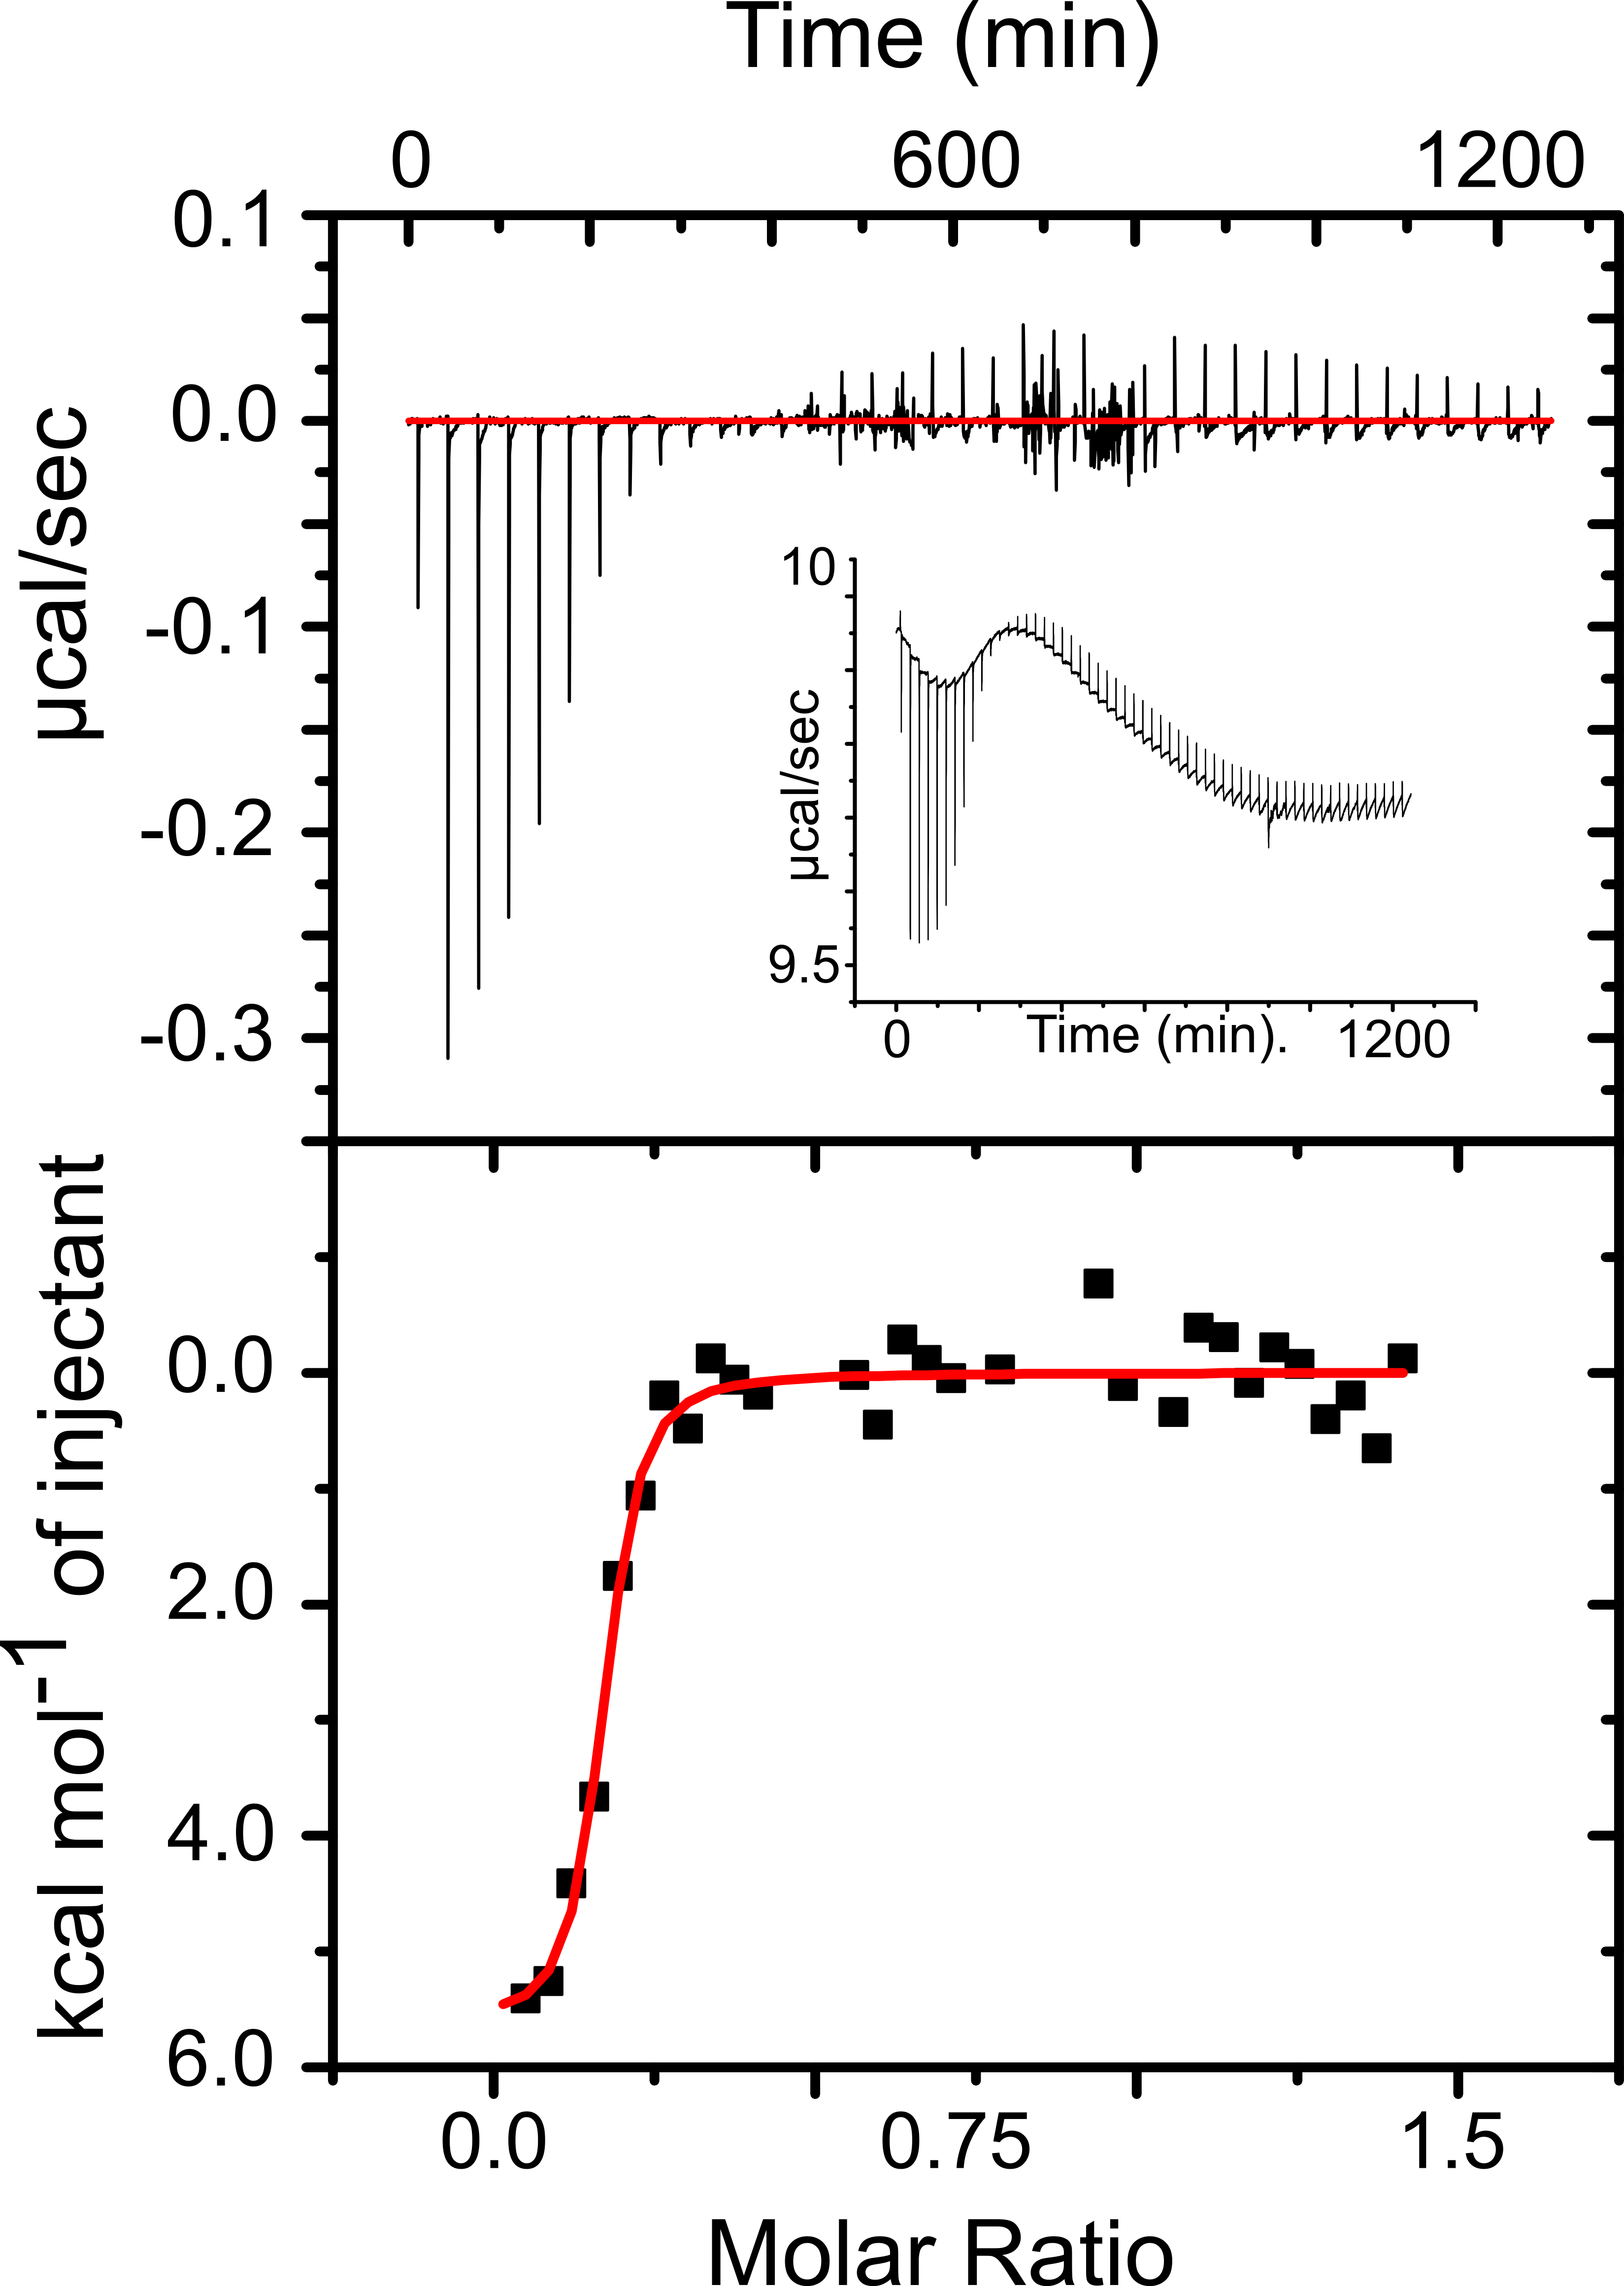
\includegraphics{ch4-fig1.png} 
\caption[Measurements of Cu\textsuperscript{2+} binding to
wildtype S100A5 in the presence\newline of Ca\textsuperscript{2+} are difficult
to interpret]{Measurements of Cu\textsuperscript{2+} binding to
wildtype S100A5 in the presence of Ca\textsuperscript{2+} are difficult
to interpret. Representative ITC trace showing Cu\textsuperscript{2+} 
titrated onto Ca\textsuperscript{2+}-bound wildtype S100A5. Inset
shows raw data trace. Data were characteristically noisy and the apparent
fraction competent was systematically low.\label{samplefigure}}	
\end{figure}


We found previously that neither of the two native Cys residues in
S100A5 were required for Cu\textsuperscript{2+} binding \cite{wheeler_multiple_2016}.
We also noticed that---unlike the wildtype protein---the Cys-free mutant
did not precipitate in the presence of saturating Ca\textsuperscript{2+} 
and Cu\textsuperscript{2+}. We thus sought to use ITC to characterize
the interaction between binding of the two metal ions using the Cys-Ser
double mutant. Because some of the metal-binding curves were complex
and difficult to fit, we used a Bayesian Markov Chain Monte Carlo
sampler---as implemented in pytc---to estimate thermodynamic parameters
for all binding models \cite{noauthor_pytc:_2017}. We also included
a floating ``fraction competent'' parameter to capture uncertainty
in the relative protein and metal concentrations (following SEDPHAT
\cite{zhao_sedphat_2015}). This was necessary because a number of
factors make it difficult to obtain accurate estimates of concentrations
for components of this system. S100A5 has no tryptophan residues and,
therefore, a low extinction coefficient that makes absorbance-based
concentration estimates unreliable. Further, water absorption by dry
metal salts, as well as interactions between metal ions and buffer,
can also make estimates of metal concentration difficult. Because
of these of uncertainties, ITC has been noted to provide poor estimates
of stoichiometry for protein metal binding \cite{zhang_isothermal_2000}. 

We first used ITC to remeasure binding of Cu\textsuperscript{2+} 
ions to the apo form of the S100A5 double mutant. We found the Cu\textsuperscript{2+} 
binding data was best described with a single-site binding model.
In line with our previous observations, the protein bound Cu\textsuperscript{2+} 
with a $K_{d}$($\mu M$) that had a 95\% credibility region of $0.94\le1.81\le3.90$
(Figure 11A, Table 1). We next measured the binding of Cu\textsuperscript{2+} 
in the presence of saturating Ca\textsuperscript{2+}. Ca\textsuperscript{2+} 
had no detectable effect on the binding of Cu\textsuperscript{2+} 
to the protein, giving a $K_{d}$($\mu M$) of $0.65\le0.96\le1.47$
(Figure 11B; Table 1). 

\begin{figure}
\centering
	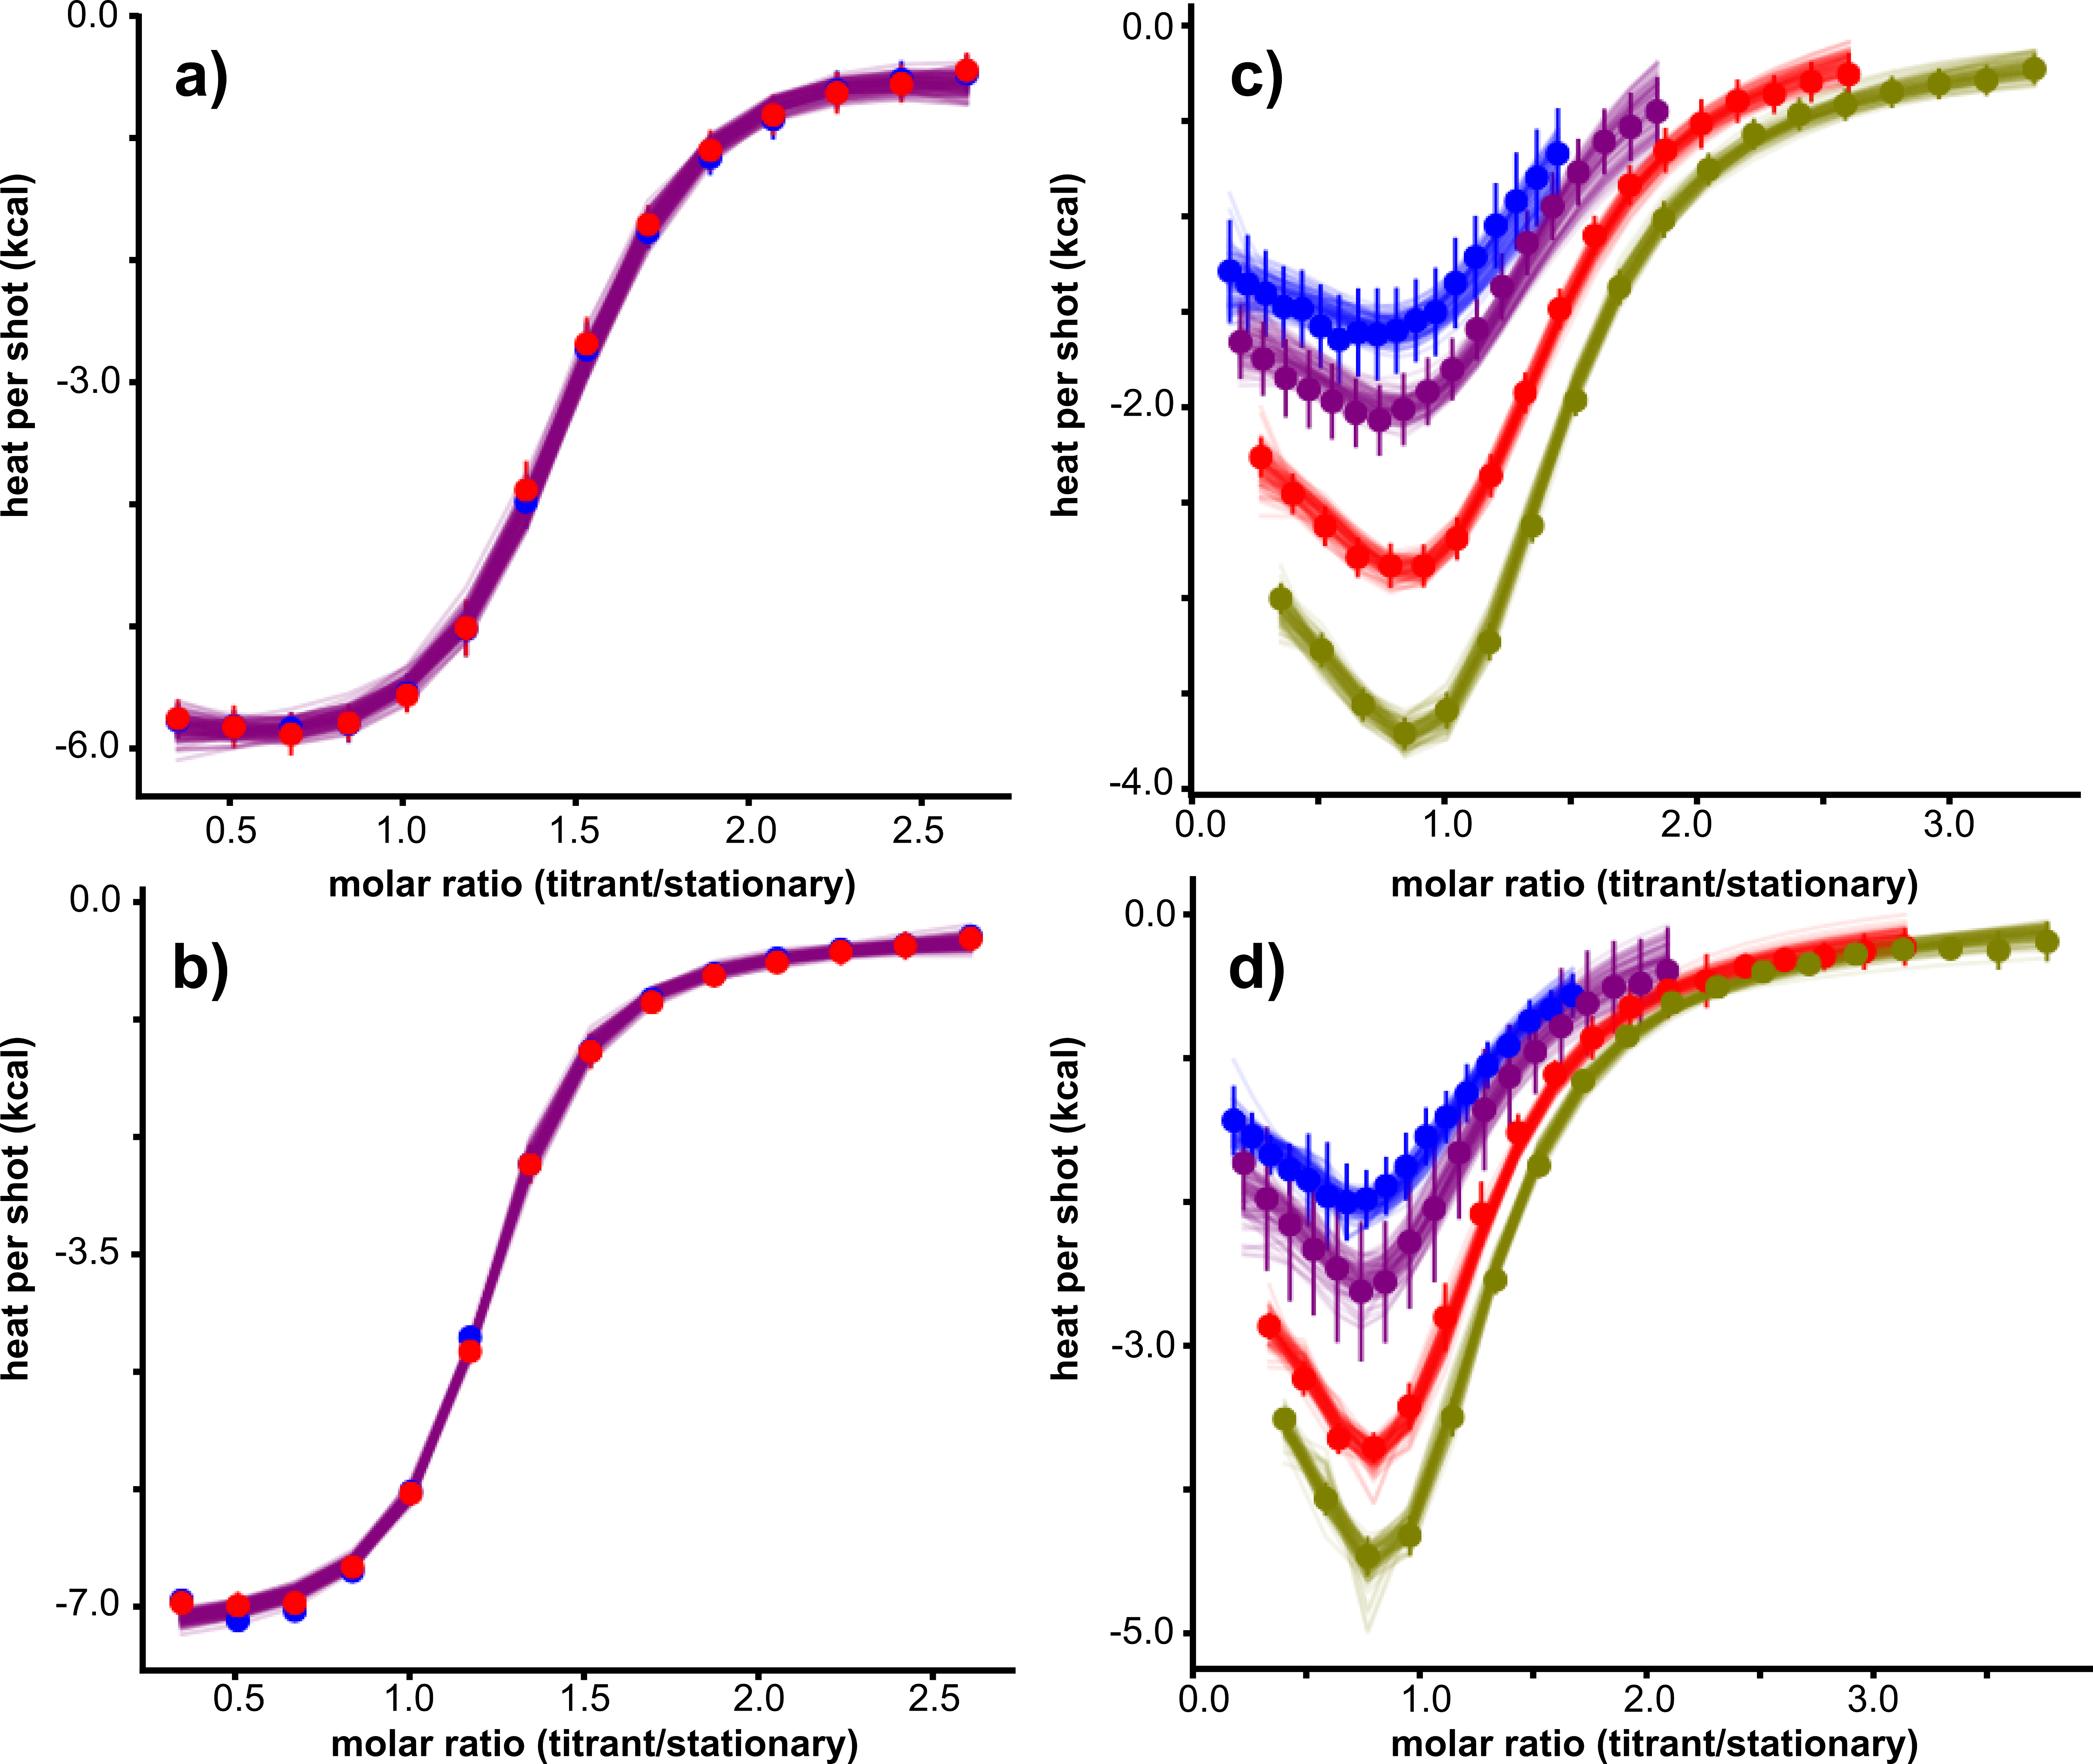
\includegraphics{ch4-fig2.png} 
\caption[S100A5 can bind Ca\textsuperscript{2+} and Cu\textsuperscript{2+} 
without antagonism]{S100A5 can bind Ca\textsuperscript{2+} and Cu\textsuperscript{2+} 
simultaneously without antagonism. Plots show integrated data and
global Bayesian fits from replicate isothermal titration calorimetry
experiments: a) Cu\textsuperscript{2+} binding to apo protein, b)
Cu\textsuperscript{2+} binding to Ca\textsuperscript{2+}-saturated
protein, c) Ca\textsuperscript{2+} binding to apo protein, and d)
Ca\textsuperscript{2+} binding to Cu\textsuperscript{2+}-saturated
protein. Points are integrated titration shots. Lines are 100 curves
drawn from the posterior distribution of the MCMC samples. For Cu\textsuperscript{2+} 
binding experiments technical replicates are shown in blue and red.
Ca\textsuperscript{2+} binding experiments were performed with fixed
protein concentration and four different titrant/titrate ratios: 8X
(blue), 10X (purple), 15X (red), and 18X (green). For clarity Y-axes
display total heat per shot, so that curves from different titrant
concentrations fall on different areas of the graph. Raw data corresponding
to these integrated heats are displayed in figure 31 in supplement.\label{samplefigure}}	
\end{figure}

We next performed the inverse set of experiments. We used ITC to measure
the binding of Ca\textsuperscript{2+} to the protein in the apo and
Cu\textsuperscript{2+} –saturated forms. For each condition, we used
four different titrant/stationary ratios to better resolve the complex
Ca\textsuperscript{2+} binding curve and then globally fit a binding
model to all four datasets (Figure 11C). This binding curve had two
distinct phases and could be fit with a two-site binding polynomial
(Figure 11C). These Ca\textsuperscript{2+} binding curves presented
a challenging model-fitting problem due to the complex shape of the
curve. The individual enthalpies and binding constants may therefore
be under-determined in our analysis. To resolve realistic parameter
values from the binding polynomial model, we constrained the dilution
heat and dilution intercept in the Bayesian fit to reasonable values. 

\begin{table}[h!]\footnotesize
\caption[Fit parameters from pytc Bayesian fits] {Table contains values
for key parameters determined via global fits of ITC data using the
Bayesian MCMC fitter in pytc. 95\% credibility regions from the posterior
distributions are reported for parameter values. $\Delta H$ values
are reported in $kcal\cdot mol^{-1}$, $K_{d}$ values in $\mu M$.
Final parameter is fraction competent, a nuisance parameter that captures
what fraction of the metal and protein in solution are competent for
the measured reaction.}
\scriptsize
\begin{tabular}{c|cc|cc}
ion & \multicolumn{2}{c|}{$Cu^{2+}$} & \multicolumn{2}{c}{$Ca^{2+}$}\tabularnewline\hline 
competitor & none & $Ca^{2+}$ & none & $Cu^{2+}$\tabularnewline 
\hline 
$\Delta H_{1}$ & $-5.7\le-3.4\le-2.8$ & $-4.1\le-3.6\le-3.2$ & $-1.8\le-1.4\le-0.7$ & $-1.5\le-1.2\le-0.7$\tabularnewline
$\Delta H_{2}$ & --- & --- & $-5.7\le-4.6\le-3.7$ & $-5.0\le-4.1\le-3.4$\tabularnewline
$K_{d,1}$ & $0.9\le1.8\le3.9$ & $0.7\le1.0\le1.5$ & $0.4\le0.5\le2.7$ & $0.03\le0.2\le2.2$\tabularnewline
$K_{d,2}$ & --- & --- & $1.9\le6.3\le34.9$ & $1.9\le10.5\le100$\tabularnewline
fx. comp. & $1.40\le1.43\le1.47$ & $1.15\le1.17\le1.19$ & $0.61\le0.66\le0.69$ & $0.54\le0.58\le0.61$\tabularnewline
\end{tabular}
\end{table}


We observed one high-affinity site ($K_{d}$($\mu M$): $0.14\le0.46\le2.68$)
and one lower-affinity site ($K_{d}$($\mu M$): $1.85\le6.33\le34.88$).
The values were roughly consistent with those reported in the literature
\cite{kim_biophysical_2017}. The presence of saturating Cu\textsuperscript{2+} 
did not inhibit the binding of Ca\textsuperscript{2+} ions (Figure
11D; Table 1). The $K_{d}$ value of the low affinity site ($K_{d}$($\mu M$):
$0.03\le0.18\le2.16$) was not distinguishable within uncertainty
from that of the apo protein. The $K_{d}$ of the high affinity site
($K_{d}$($\mu M$): $1.86\le10.46\le100.3$) is similarly indistinguishable
from that for the apo protein (Table 1). Our results clearly demonstrate
that Ca\textsuperscript{2+} and Cu\textsuperscript{2+} ions do not
display strong antagonism when binding to S100A5.

\subsection{S100A5 is prone to oligomerization and metal-driven aggregation}
We hypothesized that the metal-driven aggregation process observed 
in our ITC experiments with the wildtype protein contributed to the
apparent antagonism that was previously reported. To further examine
this aggregation process we used sedimentation velocity AUC to test
for the presence of oligomers in solution. We hypothesized that the
oligomerization of the wildtype protein was driven by the presence
of Cysteine residues. Due to the presence of Cu\textsuperscript{2+} 
in some samples we were unable to use a reducing agent in either the
ITC or AUC experiments. 

We performed sedimentation velocity AUC experiments on both the wildtype
and Cys-Ser double mutant proteins in both the apo form and the form
loaded simultaneously with Cu\textsuperscript{2+} and Ca\textsuperscript{2+}.
We fit the Lamm equation to the sedimentation data using SedFit to
calculate the c(s) distribution of the protein in each condition \cite{schuck_size-distribution_2000,brown_macromolecular_2006}.
We found that apo S100A5 formed high-ordered oligomers, ranging to
at least dodecamers (Figure 12A). Addition of Cu\textsuperscript{2+} 
and Ca\textsuperscript{2+} caused a large amount of precipitation
in wildtype S100A5 that we removed by extensive centrifugation prior
to loading the cell. The remaining soluble protein was indistinguishable
from the apo protein (Figure 12). In contrast, when we performed the
same experiments with the Cys-Ser double mutant we found that the
protein was primarily dimeric in solution (Figure 12C, 12D), even with
the addition of Cu\textsuperscript{2+} and Ca\textsuperscript{2+}.
However, monomers were also detectable in the double mutant samples.
The monomer peak appears to be more prominent in the apo-protein sample
than in the sample saturated with Cu\textsuperscript{2+} and Ca\textsuperscript{2+},
suggesting that binding of metals may stabilize the dimeric form (Figure
12C, 12D). Our AUC results clearly demonstrate that oligomerization
of S100A5 is driven by the native cysteine residues, which also likely
cause the visible aggregation we observed in the ITC experiments.
This observation strongly suggests that the previously-reported apparent
antagonism between Ca\textsuperscript{2+} and Cu\textsuperscript{2+} 
was due to oligomerization and/or aggregation.

\begin{figure}
\centering
	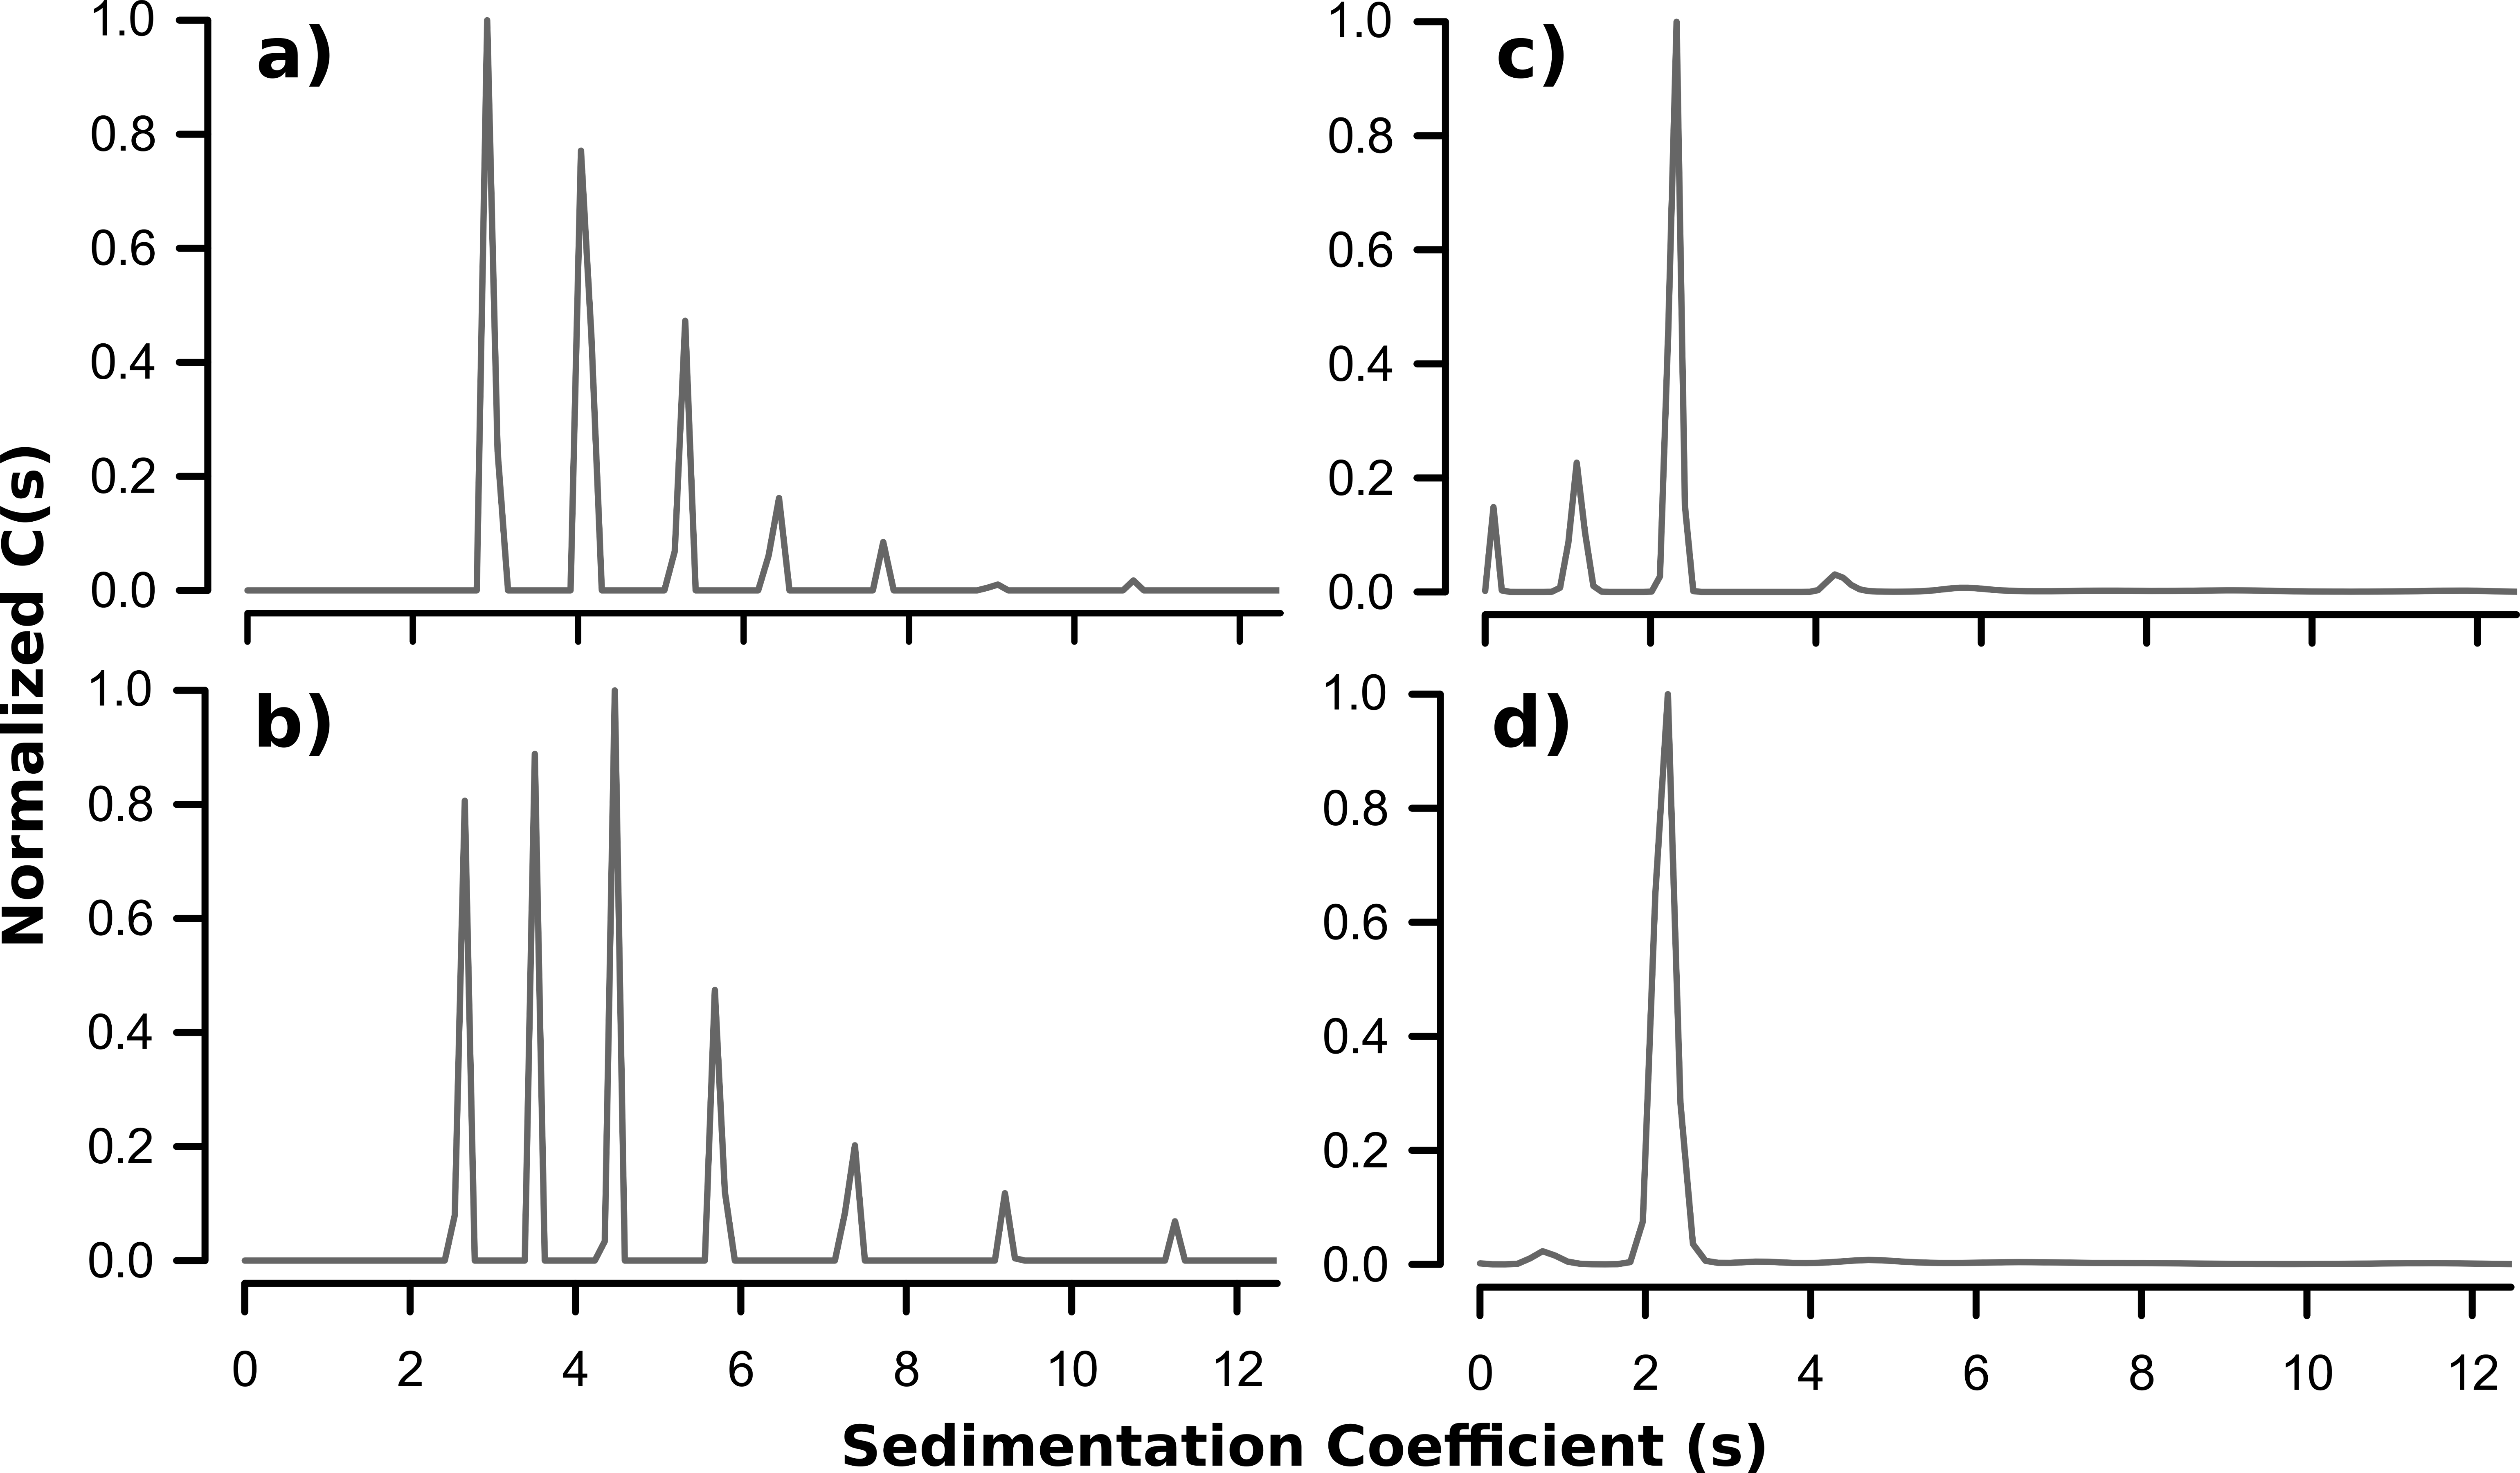
\includegraphics{ch4-fig3.png} 
\caption[Wildtype S100A5 forms high-ordered
oligomers]{Wildtype S100A5 is prone to the formation of high-ordered
oligomers. Sedimentation velocity AUC distribution plots showing
a) apo wildtype S100A5, b) wildtype S100A5 saturated with Cu\textsuperscript{2+}
and Ca\textsuperscript{2+}, c) apo Cys-Ser double mutant, and d)
Cys-Ser double mutant saturated with Cu\textsuperscript{2+} and Ca\textsuperscript{2+}.
Data are normalized to the same scale. Homodimers are the peaks near
$s=2$. The Cys-Ser double mutant plots show evidence of some monomer
(peak near $s=1$) in solution.\label{samplefigure}}	
\end{figure}

\subsection{Binding of Ca\protect\textsuperscript{2+} and Cu\protect\textsuperscript{2+} 
induce reversible changes in S100A5 secondary structure}

One hallmark feature of the S100 proteins is the change in secondary
structure observed upon binding of metal ions \cite{wheeler_multiple_2016,bertini_solution_2012,sturchler_s100a16_2006}.
Metal-induced conformational changes expose a binding interface that
can bind downstream targets and regulate their activities \cite{santamaria-kisiel_calcium-dependent_2006,kim_biophysical_2017}.
In the original publication on S100A5 biochemical characterization,
the authors found that the secondary structure of the protein is insensitive
to the binding of metal ions \cite{schafer_brain_2000}. However,
we previously found that binding of Ca\textsuperscript{2+} ions to
wildtype S100A5 induces a significant ($\approx$25\%) reversible
increase in $\alpha$-helical secondary structure, which is consistent
with the changes observed in published NMR data \cite{bertini_solution_2009,kim_biophysical_2017}.
Due to instantaneous sample precipitation, we were unable to reliably
measure structural changes of wildtype S100A5 in the presence of Cu\textsuperscript{2+}.
However, the Cys-Ser double mutant protein alleviates this issue.
We collected far-UV circular dichroism spectra of the mutant protein
in the apo form and bound to Ca\textsuperscript{2+}, Cu\textsuperscript{2+},
and Ca\textsuperscript{2+} and Cu\textsuperscript{2+} simultaneously.
The Cys-Ser mutant displays a notable increase in alpha-helical signal
(222nm) upon binding of Ca\textsuperscript{2+}, identical to the
wildtype protein. Interestingly, addition of Cu\textsuperscript{2+} 
also induces an increase in $\alpha$-helical signal that is approximately
half of that induced by Ca\textsuperscript{2+}. The spectrum of S100A5
bound simultaneously to both metals is identical to that of the Ca\textsuperscript{2+}-bound
form (Figure 13). This structural change is not due to oligomerization,
as the protein remains a dimer under these conditions by AUC (Figure
13D). All the metal induced structural changes were instantly reversible
by the addition of a molar excess of EDTA. These results may help
to explain the minor differences---such as larger enthalpy---in Ca\textsuperscript{2+} binding
to the Cu\textsuperscript{2+} –bound form of the protein, which may
be due to moderate structural differences from the apo-protein. Despite
the lack of antagonism between binding affinities for Ca\textsuperscript{2+} 
and Cu\textsuperscript{2+} ions, there is still indication of some
structural interplay between the two metals.

\begin{figure}
\centering
	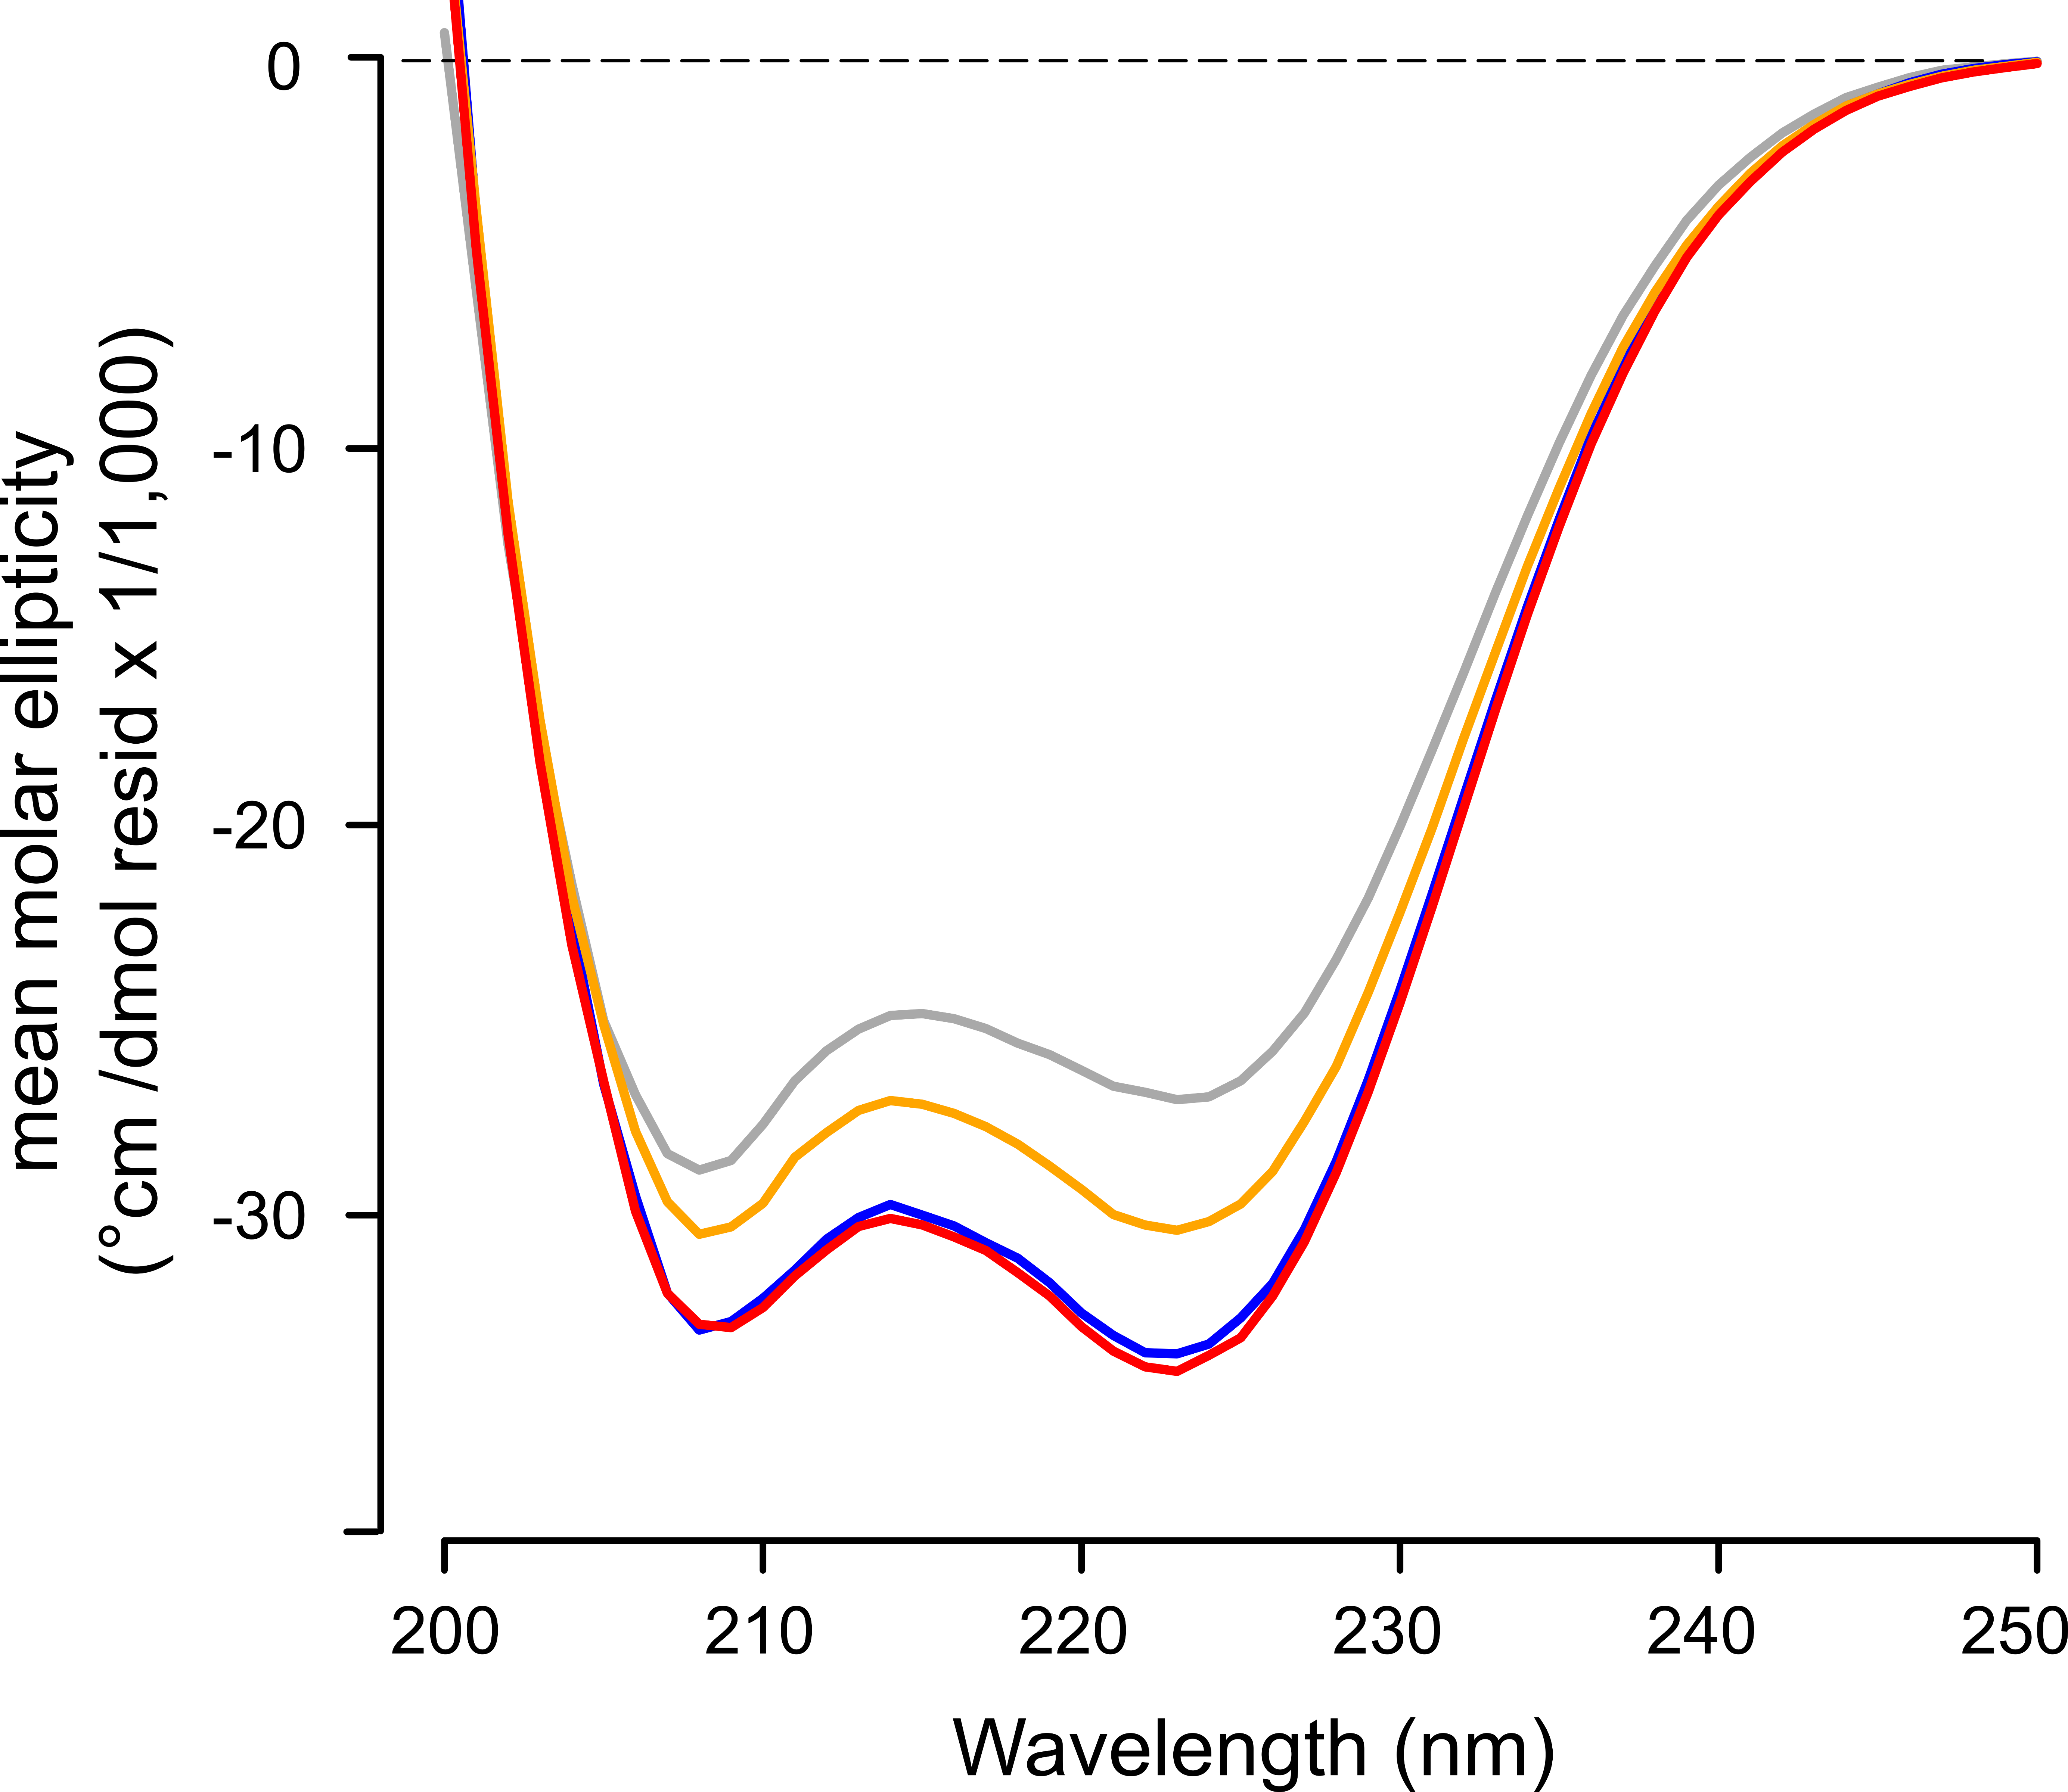
\includegraphics{ch4-fig4.png} 
\caption[Ca\textsuperscript{2+} and Cu\textsuperscript{2+} 
induce increases in $\alpha$-helical secondary structure\newline measured
by far UV circular dichroism]{Ca\textsuperscript{2+} and Cu\textsuperscript{2+} 
induce increases in $\alpha$-helical secondary structure measured
by far UV circular dichroism. Curves show mean molar ellipticity
vs. wavelength for each experimental condition: Apo (gray), bound
to Cu\textsuperscript{2+} (orange), bound to Ca\textsuperscript{2+} 
(blue), and bound to both Cu\textsuperscript{2+} and Ca\textsuperscript{2+} 
(red).\label{samplefigure}}	
\end{figure}

\section{Discussion}
S100A5 is one of the lesser-known members of the S100 protein family.
Its expression pattern is very narrow and its biological functions
are mostly uncharacterized. However, it has been the target of multiple
biochemical studies that have sought to characterize the properties
of the protein itself. Binding of metals and proteins to S100A5 have
been studied using various techniques \cite{schafer_brain_2000,wheeler_multiple_2016,bertini_solution_2009,cho_pentamidine_2016,kim_biophysical_2017}.
X-ray crystallography and NMR have been used to solve structures of
both apo and Ca\textsuperscript{2+} –bound forms of the protein \cite{bertini_solution_2009,liriano_protein_nodate}.
Despite the available biochemical data aspects of S100A5 have remained
ambiguous. For example, the stoichiometry of transition metal binding
and structural responses to metal binding have been variably reported
\cite{schafer_brain_2000,wheeler_multiple_2016}. 

One of the most noted features of S100A5 is the strong antagonism
between binding of Ca\textsuperscript{2+} and Cu\textsuperscript{2+} ions.
This feature is reported in the gene descriptions found in many databases
\cite{noauthor_s100a5_nodate,noauthor_s100a5_nodate-1,noauthor_wikigenes_nodate}.
In this study we set out to characterize this unique feature of S100A5,
hypothesizing that it was due to competition between the two metals
for shared ligands. However, we found an absence of direct binding
antagonism between Ca\textsuperscript{2+} and Cu\textsuperscript{2+}.
Neither metal ion affects the binding constant for the other. Instead,
we observed a propensity of the protein for oligomerization and metal-induced
aggregation. It is possible that the reduction of binding-competent
protein caused by this aggregation process was interpreted in the
original flow dialysis study of S100A5 as antagonism between Ca\textsuperscript{2+} 
and Cu\textsuperscript{2+}. We also report notable changes in the
secondary structure of S100A5 upon binding of both Ca\textsuperscript{2+} 
and Cu\textsuperscript{2+}, which is contrary the original report
that S100A5 structure is insensitive to the binding of metals. 

One intriguing implication of our observations is that the Cu\textsuperscript{2+} 
binding site of S100A5 must be quite distinct from that of other S100
proteins. Ca\textsuperscript{2+} and Cu\textsuperscript{2+} clearly
do not share ligands, or there would be evidence of competition in
our ITC experiments. Cysteine residues are thought to be involved
in metal-binding in some other S100s \cite{koch_implications_2007,moroz_role_2010}
and we previously showed that the Cys-free mutant of S100A5 displays
compromised Zn\textsuperscript{2+} binding \cite{wheeler_multiple_2016}.
However, neither native Cys residue of S100A5 is required for Cu\textsuperscript{2+} 
binding. Furthermore, we showed that Zn\textsuperscript{2+} and Cu\textsuperscript{2+} 
do not share ligands, as they do not compete at all in ITC experiments
\cite{wheeler_multiple_2016}. In addition, mutation of His17---which
is present in the canonical transition metal site of many S100s---also
had no effect on Cu\textsuperscript{2+} binding in S100A5 \cite{wheeler_multiple_2016}.
The results presented here with the Cys-free mutant also clearly rule
out the possibility of oligomer-dependent Cu\textsuperscript{2+} 
binding, such as could be achieved by the formation of a new site
in a high-order oligomeric species. Thus, we still have no clues as
to where Cu\textsuperscript{2+} ions bind on S100A5. Further characterization---such
as via scanning mutagenesis---will be necessary to determine the identity
of Cu\textsuperscript{2+} ligands.

Biological roles for the binding of transition metals have been established
for some S100s and suggested for many others \cite{moroz_role_2010,gilston_binding_2016,damo_molecular_2013,koch_implications_2007,sivaraja_copper_2006}.
The binding constants that we measured for Ca\textsuperscript{2+} 
and Cu\textsuperscript{2+} suggest the possibility of physiologically
relevant interactions in some tissues. Free Ca\textsuperscript{2+} 
concentrations in rat olfactory neurons reach $\approx2\ \mu M$ during
nerve stimulation \cite{reisert_ca-activated_2003}. Likewise, pools
of Cu\textsuperscript{2+} are released in and around olfactory neurons
during signaling, reaching concentrations as high as $10\ \mu M$
in the synapse \cite{gardner_metal_2017,herms_evidence_1999,hopt_methods_2003,horning_zinc_2001}.
Further, despite high Cu\textsuperscript{2+} concentrations, the
olfactory bulb in rats does not have elevated expression of the typical
copper chaperone metallothionein \cite{ono_regional_1999}. It has
been suggested that S100A5 may play a role as a Cu\textsuperscript{2+} 
buffer or chaperone in OSNs during olfactory signaling \cite{schafer_brain_2000}.
The fact that Cu\textsuperscript{2+} is able to induce structural
changes in S100A5 suggests it could play a more active role: S100A5
could actually respond to Cu\textsuperscript{2+} and propagate a
resulting signal by interacting with downstream targets. 

Due to lack of antagonism, Cu\textsuperscript{2+} –dependent functions
could be achieved even in the presence of saturating Ca\textsuperscript{2+} levels.
Furthermore, there could be synergistic functional roles for binding
of Ca\textsuperscript{2+} and Cu\textsuperscript{2+}. For example,
if S100A5 is acting as a Cu\textsuperscript{2+} chaperone, binding
of Ca\textsuperscript{2+} could facilitate binding of protein targets---via
exposure of the hydrophobic binding interface---to which Cu\textsuperscript{2+} 
is being delivered. Furthermore, S100A5 is capable of binding Zn\textsuperscript{2+} 
ions---which are also at high concentration in the olfactory bulb---with
similar affinity to Cu\textsuperscript{2+} \cite{horning_zinc_2001}.
Zn\textsuperscript{2+} and Cu\textsuperscript{2+} also bind noncompetitively
and thus all three metals could potentially engage in synergistic
activities \cite{wheeler_multiple_2016}. 

One final possibility is that the oligomerization process we observed
in this study may actually have a biological function. Wildtype S100A5
is prone to the formation of oligomers even in the apo form and is
subject to extensive aggregation in solutions containing Ca\textsuperscript{2+} 
and Cu\textsuperscript{2+} even at relatively low protein concentrations.
Roles for metal-driven oligomerization in S100s have been suggested
previously \cite{donato_functions_2013,streicher_modulation_2010,gribenko_oligomerization_1998,moroz_crystal_2009}.
It is conceivable that Ca\textsuperscript{2+} and Cu\textsuperscript{2+} drive
oligomerization of S100A5 in cells to facilitate a biological function,
but further experiments would be required to determine if this process
occurs in the reducing environment of the cell at physiologically-relevant
concentrations of S100A5, Ca\textsuperscript{2+} and Cu\textsuperscript{2+}.

Future experiments are needed to elucidate the biochemical features
and biological functions of S100A5 that remain unknown. It will be
important to identify the Cu\textsuperscript{2+} ligands in S100A5
to fully understand the biochemical interplay between the binding
of various biologically relevent metals. To understand how Ca\textsuperscript{2+},
Cu\textsuperscript{2+}, and Zn\textsuperscript{2+} contribute to
the biological activity of S100A5, experiments should be targeted
at directly testing how these metals interact with the protein \textit{in}
\textit{vivo}. The identification of more S100A5 biological targets
and an increase in functional studies will be required to determine
the chief roles of S100A5 in it's cellular environment. 


\section{Conclusions}

Antagonism between binding of Ca\textsuperscript{2+} and Cu\textsuperscript{2+} 
ions to S100A5 is one of the most oft-cited aspects of this protein.
Several possible biological roles have been suggested. Using careful
biophysical characterization, we discovered that binding of Ca\textsuperscript{2+} 
and Cu\textsuperscript{2+} ions is not antagonistic. A Cys-free mutant
version of the protein makes measurements of metal binding using ITC
possible and shows that the protein is capable of binding both metals
simultaneously and independently. Rather than binding antagonism,
it appears that the wildtype protein is prone to oligomerization and
aggregation and that these behaviors may have contributed to the original
interpretation. Furthermore, we also measured the effects of Ca\textsuperscript{2+} 
and Cu\textsuperscript{2+} binding on S100A5 secondary structure
and found that both metals are capable of inducing increases in $\alpha$-helical
secondary character. These results also contrast the original report
on S100A5 \cite{schafer_brain_2000}, but are consistent with previously
published NMR data \cite{bertini_solution_2009}. The ability to
bind Ca\textsuperscript{2+} and Cu\textsuperscript{2+} independently
as well as the structural response to Cu\textsuperscript{2+} may
suggest new Cu\textsuperscript{2+} –dependent biological roles for
S100A5.

\section{Methods}

\subsection{Protein expression and purification}

We previously generated the 6-histidine-tagged cysteine double-mutant
construct in a pet28/30 vector \cite{wheeler_multiple_2016}. In
this study, the protein was expressed and purified using the same
protocol detailed in the previous publication. Briefly, the protein
was expressed in a 1.5L culture of Rosetta (DE3) pLysS cells (Millipore).
Cells were lysed by sonication and treatment with DNase and lysozyme.
Subsequently, the tagged protein was purified using HisTrap Ni\textsuperscript{2+} affinity
columns (GE). The tag was then cleaved using TEV protease and the
cleaved protein was further purified using Ca\textsuperscript{2+}-dependent
hydrophobic interaction chromatography. Finally, the sample was run
over a second HisTrap Ni\textsuperscript{2+} affinity column to remove
any uncleaved protein. The purified protein was dialyzed with 6000-8000
MWCO tubing (Fisher) against 2L 25 mM Tris, 100 mM NaCl, pH 7.4 with
2g chelex resin (BioRad). The dialyzed protein was filter-sterilized
($0.22\ \mu m$), flash-frozen dropwise in liquid nitrogen, and stored
at $-80{^\circ}C$. We experimentally determined the extinction coefficient
($5002M^{-1}cm^{-1}$) of the Cys-Ser double mutant. We measured the
$A_{280}$ of the protein at the same concentration in both buffer
and denaturing 6M GdHCl (Sigma). We used ProtParam \cite{gill_calculation_1989}
to predict an extinction coefficient for the protein based on sequence
and then calculated the corrected coefficient using the equation $\varepsilon_{native}=\varepsilon_{6MGdm}\cdot A_{280,native}/A_{280,6MGdm}$.
Concentration measurements were also corrected for scattering in samples
\cite{birdsall_correction_1983}. Due to the low extinction coefficient
of the protein, concentration is difficult to measure with high confidence,
even with this careful protocol.

\subsection{Isothermal titration calorimetry}

Samples were prepared in 25 mM TES (Sigma), 100 mM NaCl (Thermo Scientific),
buffer at pH 7.4. Protein was thawed from a frozen stock and exchanged
into the experimental buffer using NAP-25 desalting columns (GE Healthcare).
For competition experiments the experimental buffer also contained
either 1 mM $CaCl_{2}$ (Sigma) or 0.25 mM $CuCl_{2}$ (Sigma). Titrant
solutions were prepared in matching experimental buffer to ensure
identical conditions to titrate. Anhydrous $CaCl_{2}$ or $CuCl_{2}$
was dissolved directly in the buffer and diluted to the appropriate
concentration immediately prior to experiments. Fresh stocks were
made for each set of experiments. Experiments were performed with
50-80 $\mu M$ protein at $25{^\circ}C$. Two technical replicates
of each Cu\textsuperscript{2+} binding experiment were performed.
To resolve the complex Ca\textsuperscript{2+} binding curves, four
Ca\textsuperscript{2+} binding experiments were performed using four
different concentrations of titrant. Raw data were integrated using
the NITPIC software package---which allows uncertainty in the baseline---and
the integrated heats were exported in standard SedPhat format \cite{keller_high-precision_2012}.
We then used the Bayesian MCMC iterator included in pytc to estimate
model parameters against all experiments simultaneously \cite{noauthor_pytc:_2017}.
We used the maximum likelihood estimate as a starting point and then
explored the likelihood surface with 100 walkers, each taking 20,000
steps. We discarded the first 10\% of steps as burn in. We restricted
parameters against all experiments simultaneously. We verified convergence
by performing the sampling procedure several times. A single site
binding model was used for Cu\textsuperscript{2+} titration data
and a two-site binding polynomial was used for Ca\textsuperscript{2+} 
titration data \cite{wiseman_rapid_1989,freire_chapter_2009}. For
Ca\textsuperscript{2+} binding fits, we constrained the dilution
heat and dilution intercept to between -3.0---0.0 kcal/mol and 0---10,000
kcal/mol/shot respectively. All other priors were uniform. 

\subsection{Sedimentation velocity analytical ultracentrifugation}

Experiments were done in 25 mM TES (Sigma), 100 mM NaCl (Thermo Scientific),
$100\ \mu M$ EDTA at pH 7.4 with the appropriate metal added directly
to the buffer during preparation. Metals were added to a final concentration
of $250\ \mu M$. Samples were prepared at $40\ \mu M$ in the appropriate
experimental buffer by overnight dialysis (6000-8000 MWCO) against
2L at $4{^\circ}C$. Before ultracentrifugation samples were centrifuged
at $18,000 \times g$ at $4{^\circ}C$ in a temperature-controlled centrifuge
for 30 minutes. Ultracentrifugation was done with sapphire windows
at $50,000 \times g$ in sector-shaped cells (Beckman) on a Beckman ProteomeLab
XL-1. Sedimentation was monitored using interference mode rather than
absorbance at 280nm due to the low extinction coefficient of S100A5.
The Lamm equation was fit to the sedimentation data---using SedFit---to
calculate the continuous c(s) distribution \cite{schuck_size-distribution_2000,brown_macromolecular_2006}.
Estimated sedimentation coefficients of the species present in solution
were calculated from the numerical fits.

\subsection{Circular dichroism spectroscopy}

Far-UV circular dichroism spectra (200–250nm) were collected on a
J-815 CD spectrometer (Jasco) with a 1 mm quartz cell (Starna Cells,
Inc.). We prepared $50\ \mu M$ samples in a Chelex (Bio-Rad) treated,
25 mM TES (Sigma), 100 mM NaCl (Thermo Scientific), $100\ \mu M$ EDTA,
buffer at pH 7.4. Samples were subsequently diluted to $25\ \mu M$
in buffers containing: no metal (apo), 1 mM Ca\textsuperscript{2+},
1 mM Cu\textsuperscript{2+}, or both 1 mM Ca\textsuperscript{2+} and
1 mM Cu\textsuperscript{2+} ---all prepared in the stock buffer above.
Samples were centrifuged at $18,000 \times g$ at $25{^\circ}C$ in a temperature-controlled
centrifuge (Eppendorf) before experiments. Spectra were collected
at $25{^\circ}C$ in a Jasco peltier multi-cell sample unit. Reversibility
of metal-induced structural changes was confirmed by adding a molar
excess of EDTA to the metal-saturated samples and repeating spectra
collection. In all cases, addition of EDTA returned the samples to
the apo state. Five scans of each condition were collected. These
scans were then averaged---using Jasco spectra analysis software---to
minimize noise. Buffer blank spectra were generated for each condition.
Applicable blanks were subtracted in the Jasco spectra analysis software.
Blank-corrected data were exported as text files and raw signal was
converted into mean molar ellipticity using the concentration and
the number of residues ($N_{res}=95$) in our S100A5 construct using
the equation: $MME=CD_{signal}/c(M)\cdot10\cdot L(cm)\cdot N_{res}$.

\section{Bridge to Chapter V}
In this chapter, the metal binding behavior of S100A5 was characterized biophysically. A misunderstood aspect of S100A5 biochemistry was resolved. It has long been thought that S100A5 exhibits strong antagonism between the binding of Ca2+ and Cu2+ ions. However, it is demonstrated here that this antagonistic behavior was likely an artifact of techniques used in the original biochemical study of S100A5. Instead, it is shown that the protein is prone to the formation of high-ordered oligomeric species. By eliminating this oligomerization process with point mutations the metal binding behavior of S100A5 could be characterized. The protein is capable of binding Ca2+ and Cu2+ ions simultaneously. Additionally, the two metals were observed to induced distinct conformational changes in the protein. This chapter is an important addition to the S100 literature, because it overturns an erroneous paradigm and suggests new biological roles for  Ca2+ and Cu2+ ion binding by S100A5. Chapter 6 turns to another basic biochemical feature of the S100 protein family; binding of small peptide regions of target proteins. Two S100 proteins, S100A5 and S100A6, that arose via gene duplication in the ancestor of amniotes are used as a model to study the diversification of binding specificity in duplicate lineages. Ancestral sequence reconstruction is used to resurrect the last common ancestor of all S100A5 and S100A6 proteins, allowing the evolutionary history of binding specificity to be directly characterized. The proteins are shown to display conserved specificity at the level of gene clades and both lineages appear to have subfunctionalized relative to the ancestor. The work in chapter VI demonstrates that proteins with low biochemical specificity nonetheless display evolutionary patterns consistent with those observed in highly-specific proteins following gene duplication. 

